\graphicspath{{Images/conclusion/}}

\chapter{conclusions and future work}
\label{chap:conclusion}
This Ph.D. research is performed as part of office of the naval research (ONR) funded project titled `Octopus-Inspired Autonomous Arms for Soft Robotics with Adaptive Motions'. The team consisted of roboticists, material scientists, and controls engineers conducted research on multiple disciplines simultaneously, which helped the informed progress of one field by considering the requirements of the other. This unique combination resulted in solving some of the key technical challenges ahead of soft robotics in general and of miniature, untethered soft robots in particular. Also, this research have some broader impact on soft robotics community and can change the way the robots are created in the future which will be discussed in this chapter.
\section{Technical and Scientific Impact}
The technical contribution of this dissertation in material science can be explained as improving the performance of PNIPAAm-based hydrogels to make them usable in soft robotic systems. These improvements include:
\begin{itemize}
 \item Increasing the speed of the hydrogel's response to the temperature changes. Prior to this improvement, the gel response was slow and therefore, no meaningful robotic movement was produced in reasonable amount of time. 
 \item Using a synthesis technique based on photopolymerization to minimize the polymerization time (to under 15 sec) and facilitate the fabrication of hydrogel structures. Prior research focused on improving the response rate without considering the ease of manufacturing and therefore the resulting gels were of less interest in the robotics community.
 \item Expanding the knowledge on underlying the mechanisms of transport phenomena in temperature-responsive hydrogles as well as the effect of their micro-structure on their response. 
 \item Expanding the knowledge on the mechanism of pore formation in hydrogels based on non cononsolvency effect. 
 \item Studying the tunability of the response of the hydrogels based on simple tweaking of ingredients. 
\end{itemize}
	
In terms of manufacturing, a bottom-up assembly approach inspired by biology has been selected to facilitate the fabrication of soft robots. Using building blocks to assemble soft robots. Building blocks can be selected from a wide range of materials. They can also contain essential components such as sensors and processors. The manufacturing of a building block is very simple and therefore they can be mass produced easily. These features facilitates the fabrication of multimaterial structures. This is critical while the range of compatible materials for 3D printing is still limited.  Inclusion of electronics in the soft robot structure would also be performed more easily.  
\subsection{Broader Impact on Soft Robotics Community}
Soft robotics has quickly turned into a broad area of research since its introduction. Therefore, new challenges have already been raised and more will be faced in the future. One of these challenges is to cut the tether from robots and enable them to operate as mobile devices. Another challenge is to reduce the size of the robots. An even tougher problem would arise when trying to solve both the aforementioned challenges simultaneously. Addressing these challenges require innovative approaches and usually requires progress in multiple fields. However, often the progress in one field is made without considering the limitations of the other fields. This problem is more profound in the field of material science regarding the development on novel materials for soft actuators and sensors. For instance, stimuli-responsive hydrogels are usually developed using complex processes and specialized equipment and therefore they are less accessible to robotics community. 

Within the field of heterogeneous hydrogel structures, the presented methods in material synthesis and manufacturing techniques have helped to achieve unique desirable features that are highly demanded in hydrogels and soft robotics research simultaneously. In the literature surveyed, individual features might have been achieved separately. However, since some of the goals are counteracting, reaching one makes the other harder to achieve. For example, improving the response rate of hydrogels is highly regarded from a materials research perspective but is often accompanied by complications in synthesis which is less favorable from a manufacturing point of view. Parallel improvements have been made through a collaboration between teams of material scientists and roboticists allowing considerations from one field to inform the other.  

In addition, by introducing the first addressable hydrogel voxels,  the field is further advanced by creating on-demand actuation and shape change of heterogeneous structures --a feature that improves the motion of a structure from hard-coded to on-demand programmable. As mentioned above, on-demand programmable shape change is one of the main goals of research in this field which is hard to achieve using the current technologies. It should be emphasized that the control signals are electrical signals, a feature inspired by biology in contrast to the previously demonstrated heterogeneous structures which use light signals or global temperature changes. Therefore, the robotic systems can be miniaturized and fully untethered simultaneously.
\subsection{Broader Impact on Society}
This research on soft robotics have many potential applications in biology, medicine and environmental science. The small footprint soft robots developed are low cost and can be manufactured in large numbers. A swarm of these robots can operate under water to collect environmental data, thanks to the intrinsic compatibility of hydrogels and water. The miniature robots can be sent inside the human body to perform drug delivery, biopsies, and tasks that require a high number of degrees of freedom in robotic manipulators.
In addition to the capability of soft robots in dealing with unstructured environment, they are intrinsically safe around humans. This can enhance the application of robots to daily life uses such as household robots and assistant robots for elderly people which are challenging using rigid robots.
\section{Future Work}
The research presented in this dissertation has opened the doors to a variety of other research opportunities. Some of these new research in the field of control of soft robots and in-depth analysis of the hydrogel materials  have already been started by different teams consisting of Ph.D., Masters and undergraduate students. An introduction to these work will be presented here and future opportunities will be discussed.
\subsection{In-depth analysis of noncosolvencey phenomenon}
While the research in this dissertation provides a method of altering the properties of  temperature-responsive PNIMPAAm hydrogels by means of mixed solvent method, the mechanisms of pore formation in this method is not fully understood. To study these mechanisms, our collaborators in the University of California, Los Angeles (UCLA) have started in-depth study of the hydrogels produced by the mixed solvent method. It is understood that the coil to globule transition of polymer chains in presence of a second solvent (Figure~\ref{fig:cononsolv}) results in the formation of pores. 
\begin{figure}[!ht]
\centering
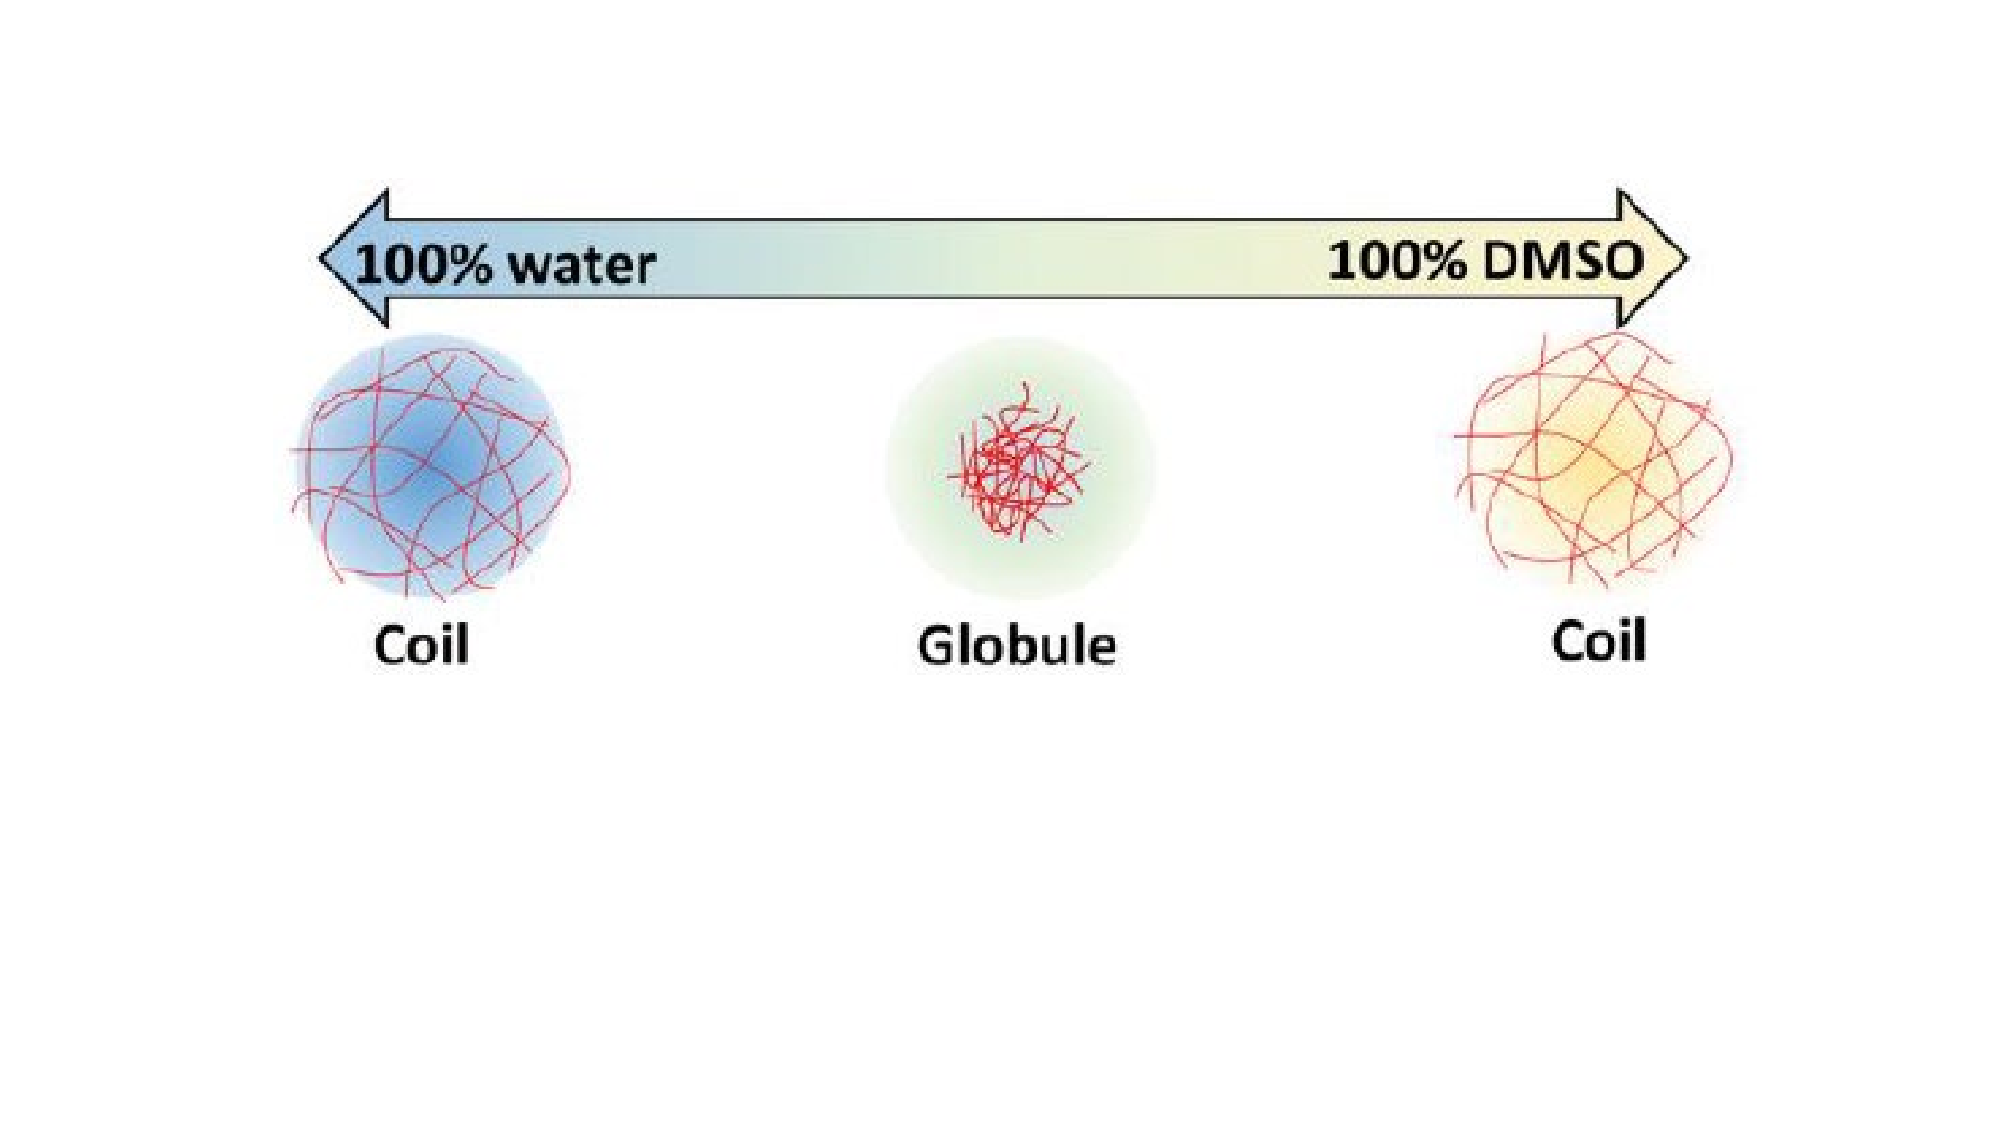
\includegraphics[width=0.7\textwidth]{cononsolv.pdf}
    \caption[]{}
    \label{fig:cononsolv}
\end{figure}

In addition, a 3D printing technique has been demonstrated. A sample 3D printed structure is shown in Figure~\ref{fig:3Dprint}. The results of this research has been accepted for publication in Advanced Materials Journal. Future work will focus on 3D printing of voxels with embedded soft heaters to remove the rigid components from the voxels and increase their production rate.
\begin{figure}[!ht]
\centering
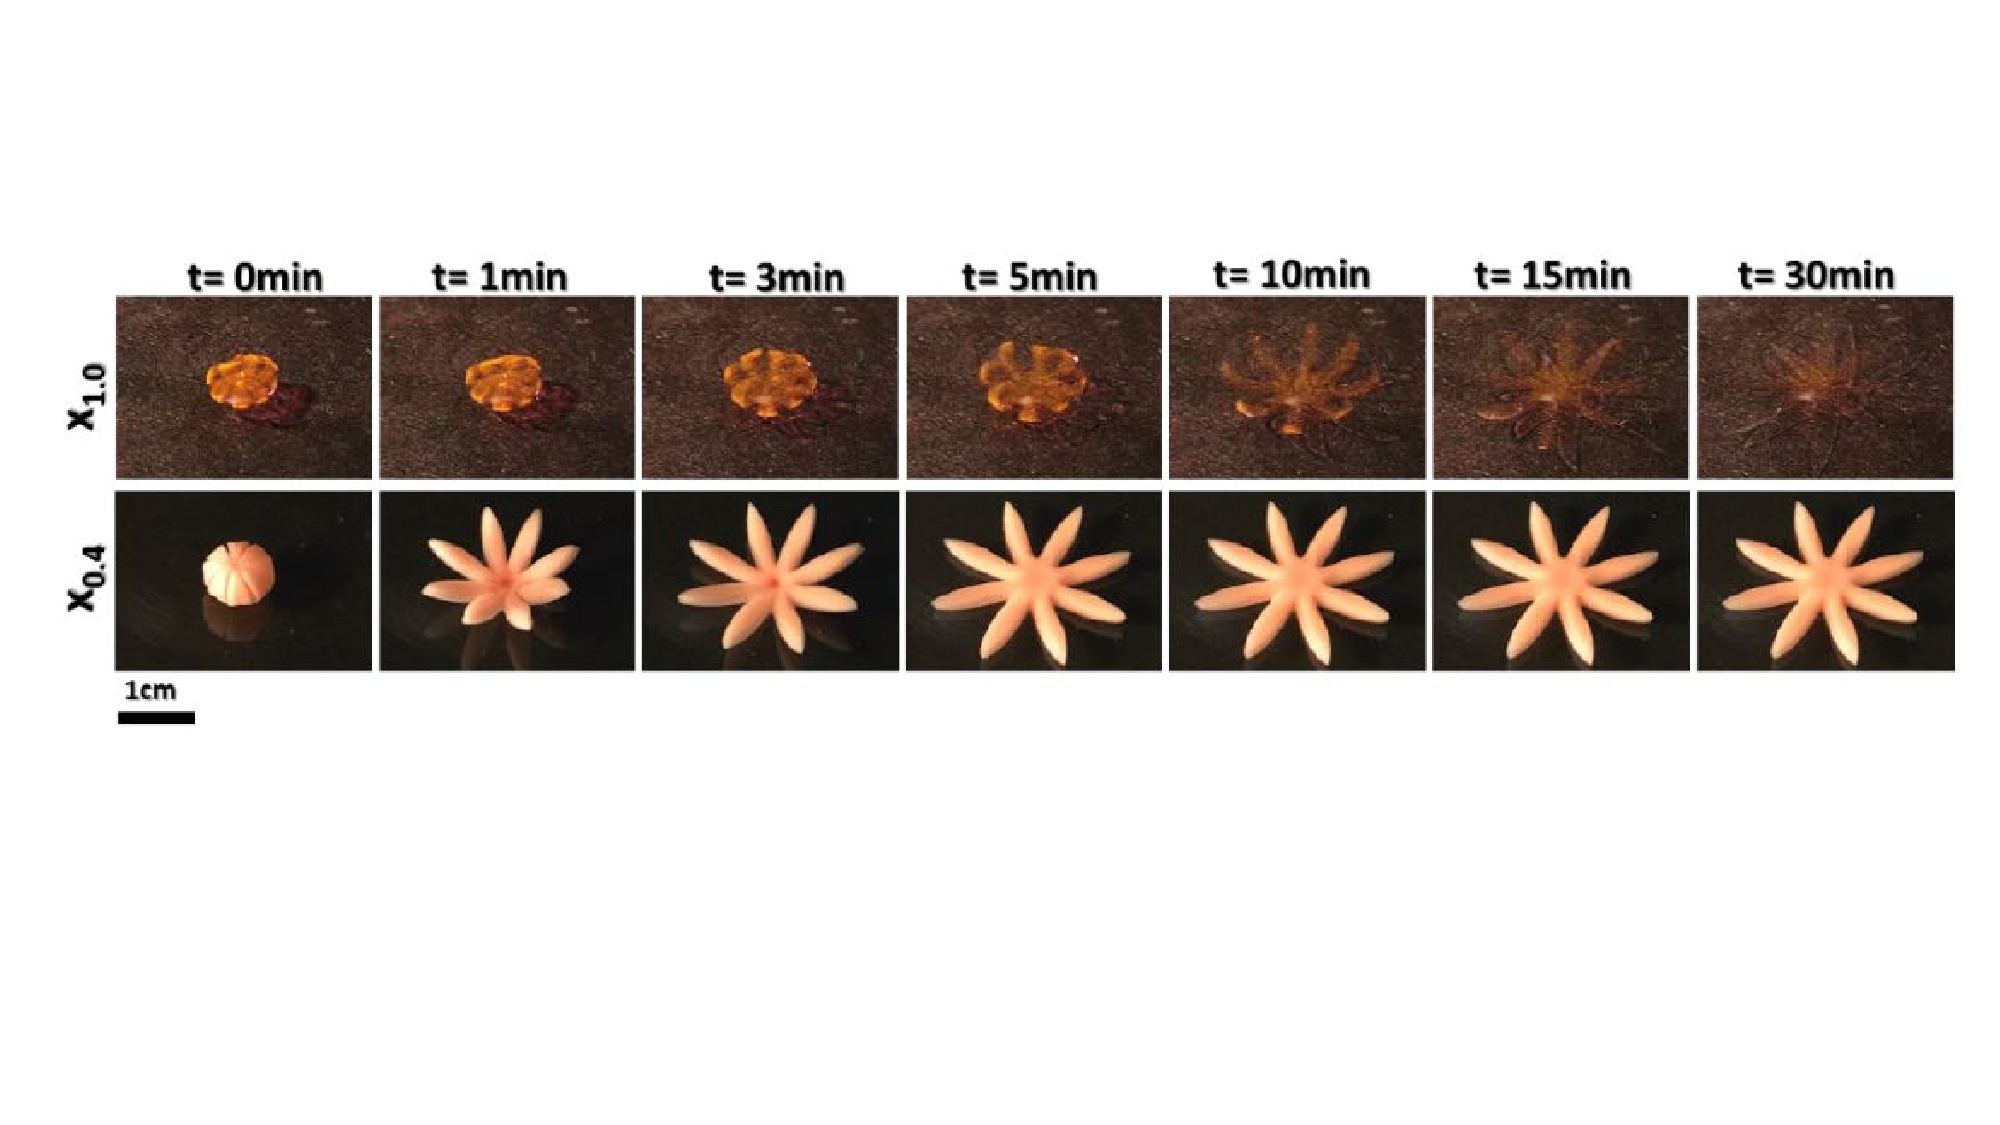
\includegraphics[width=\textwidth]{3Dprint.pdf}
    \caption[]{}
    \label{fig:3Dprint}
\end{figure}

\subsection{Control of the Hyper-redundant Robotic Arm}
\begin{figure}[!t]
\centering
\includegraphics[width=0.7\textwidth]{control.pdf}
    \caption[]{}
    \label{fig:control}
\end{figure}

\subsection{Finite Element Modeling of the Hydrogel Structures}
\begin{figure}[!t]
\centering
\includegraphics[width=0.7\textwidth]{FEM.pdf}
    \caption[]{}
    \label{fig:FEM}
\end{figure}

\subsection{Dynamic Simulation of the Voxel-based Robots}
\begin{figure}[!t]
\centering
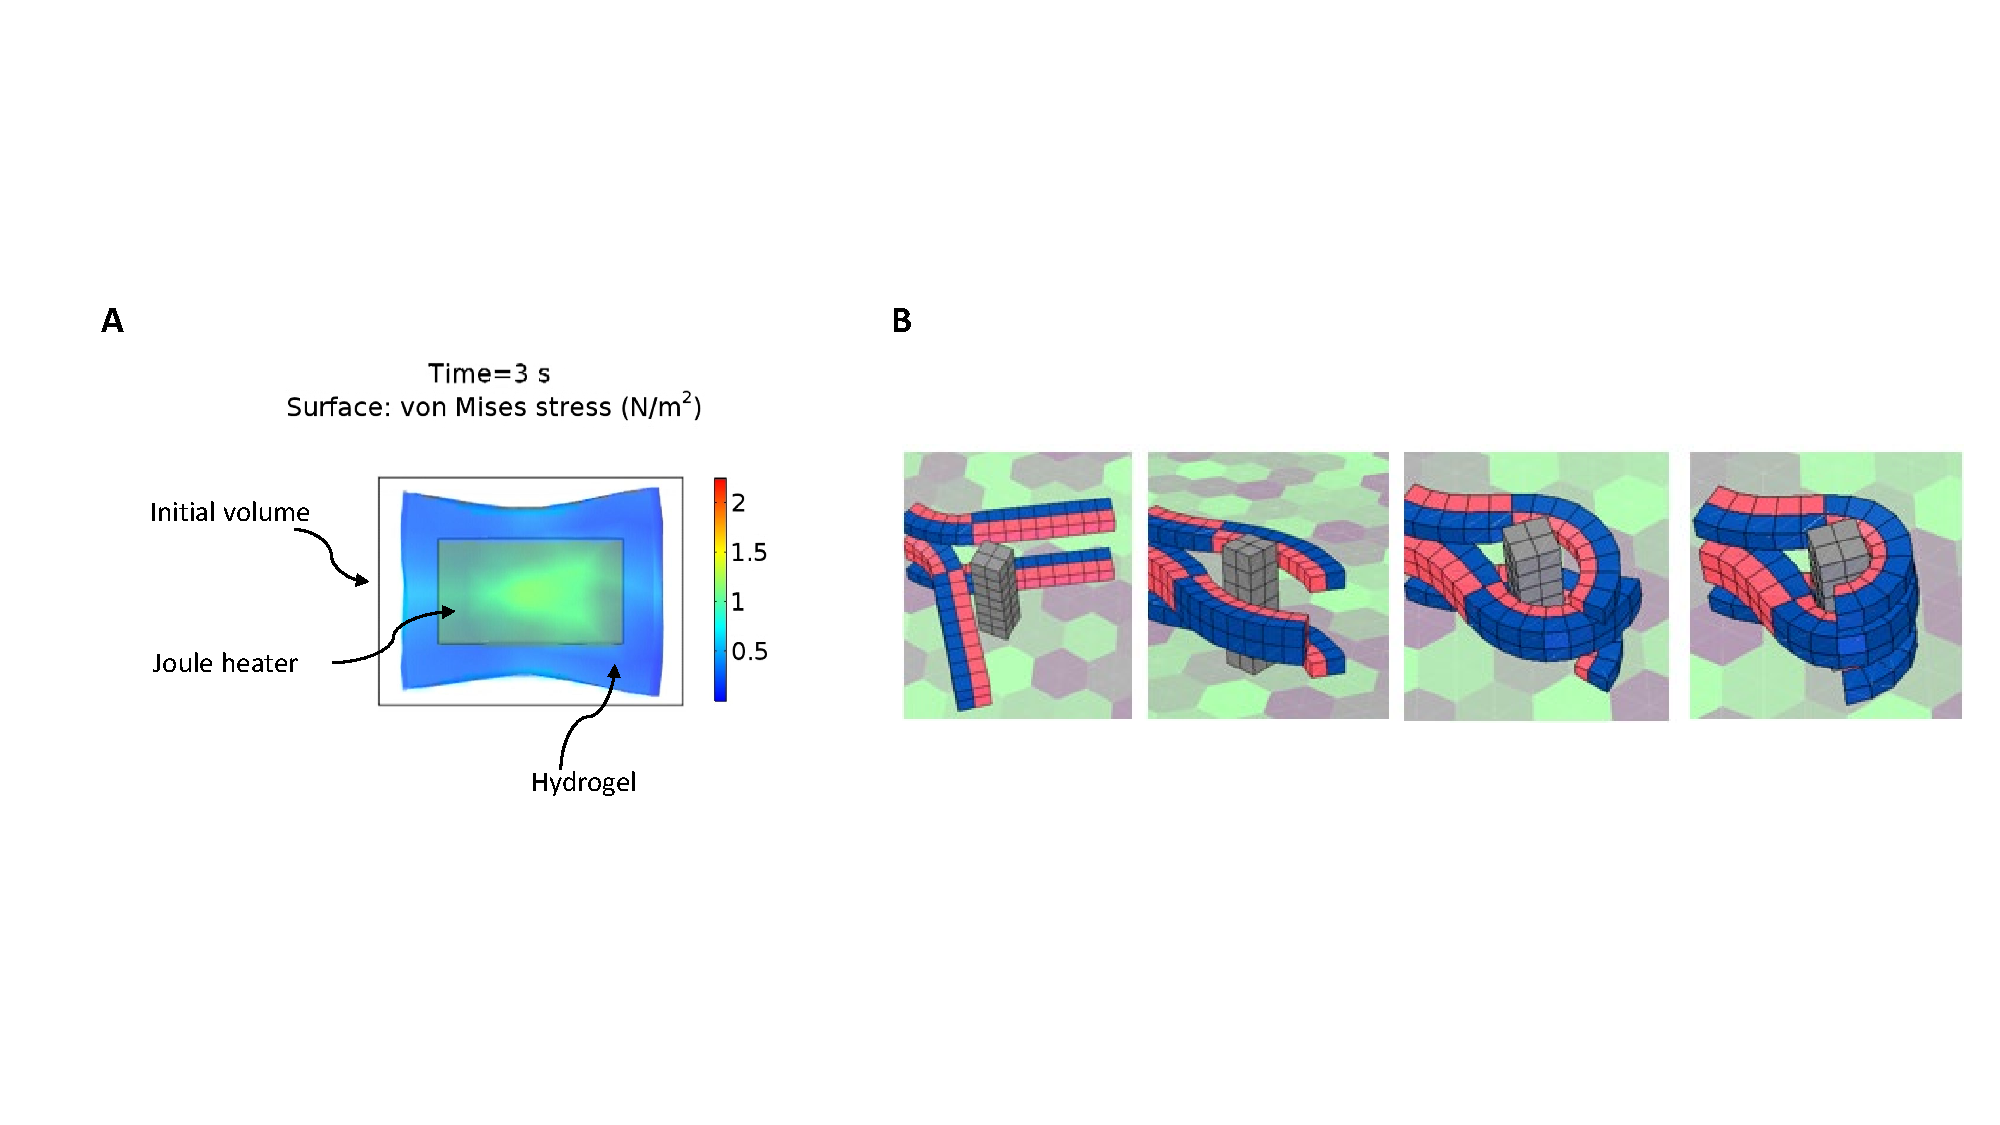
\includegraphics[width=0.7\textwidth]{voxcad.pdf}
    \caption[]{}
    \label{fig:voxcad}
\end{figure}

\subsection{A 3-dimensional prototype of the hyper-redundant robot}
\begin{figure}[!t]
\centering
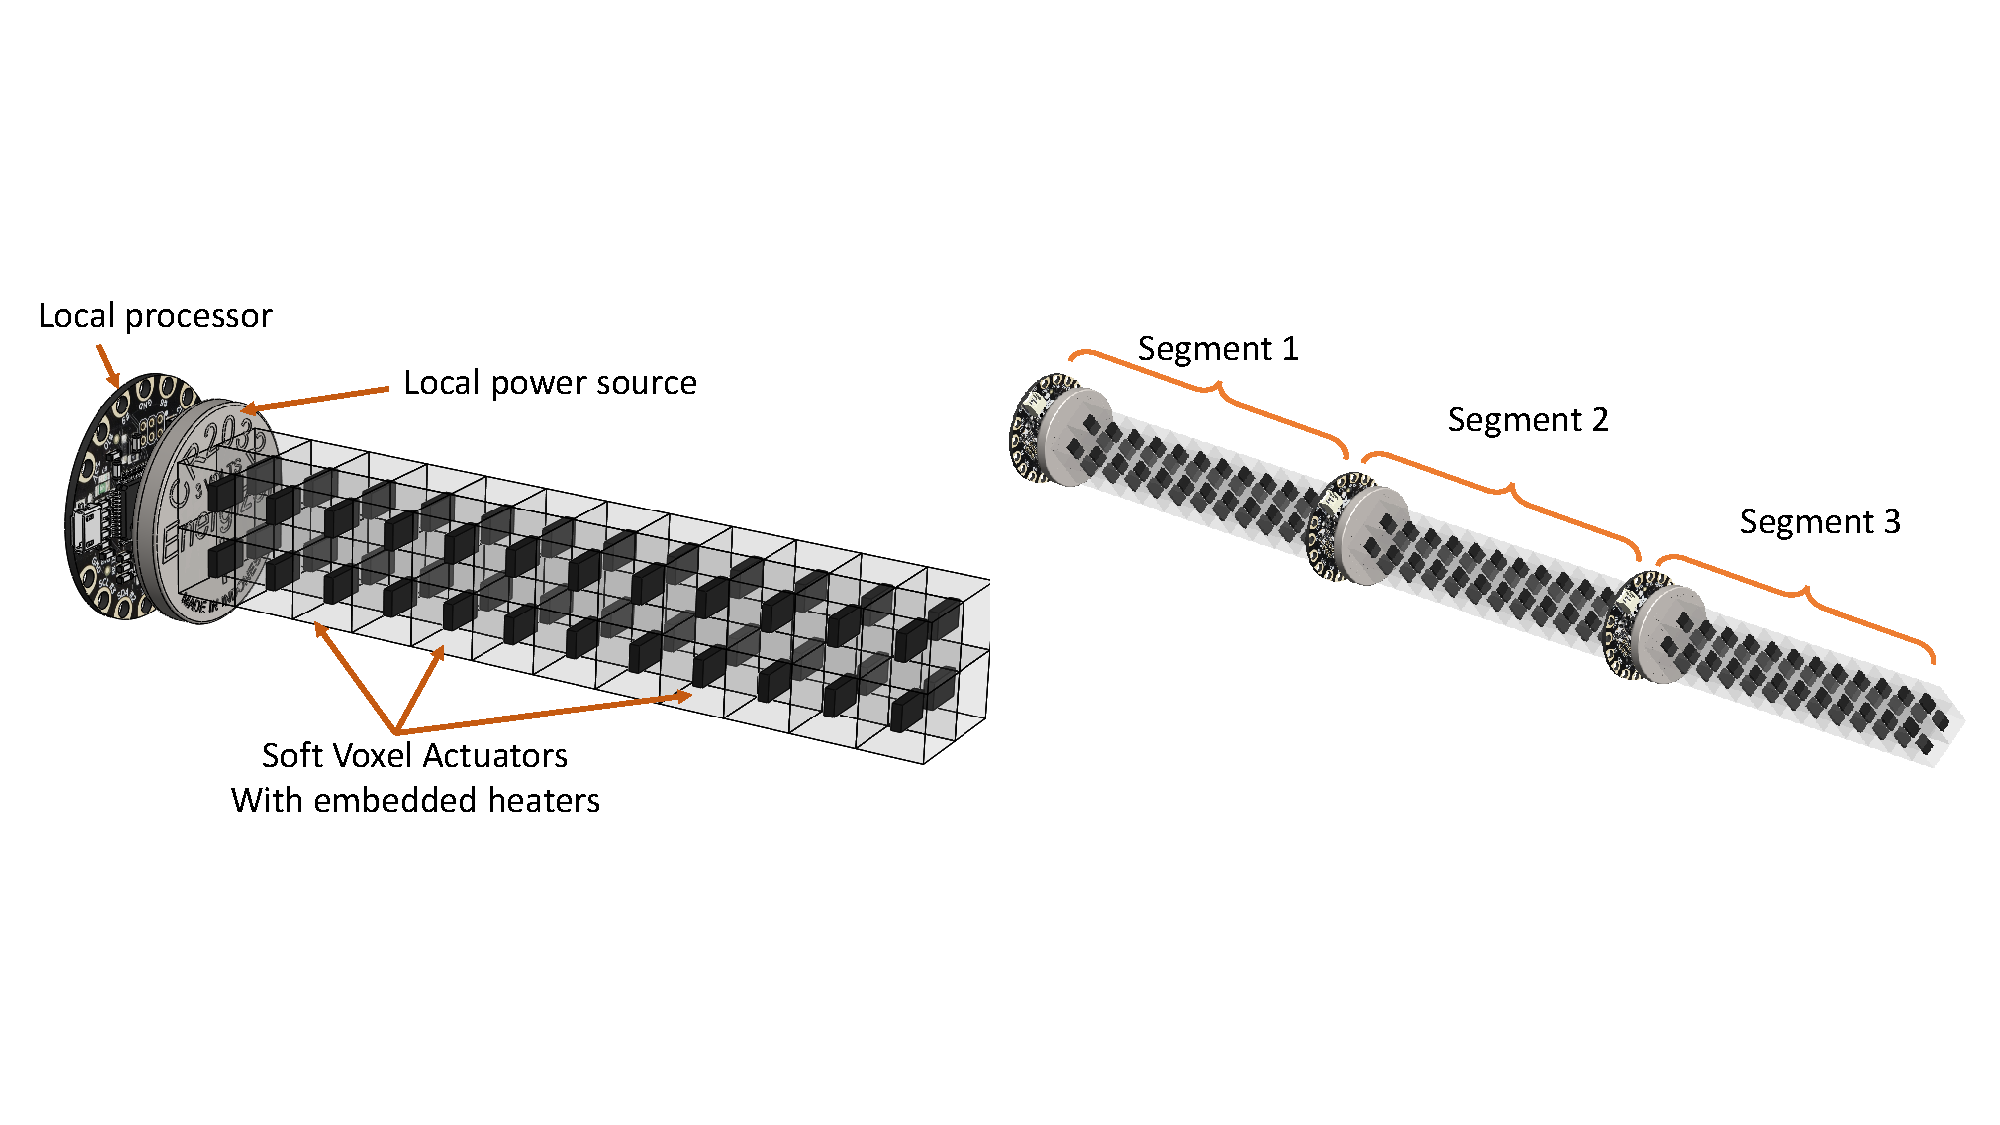
\includegraphics[width=0.7\textwidth]{3Darm.pdf}
    \caption[]{}
    \label{fig:3Darm}
\end{figure}

\subsection{Expanding the Functionality of the Robots}
\begin{figure}[!t]
\centering
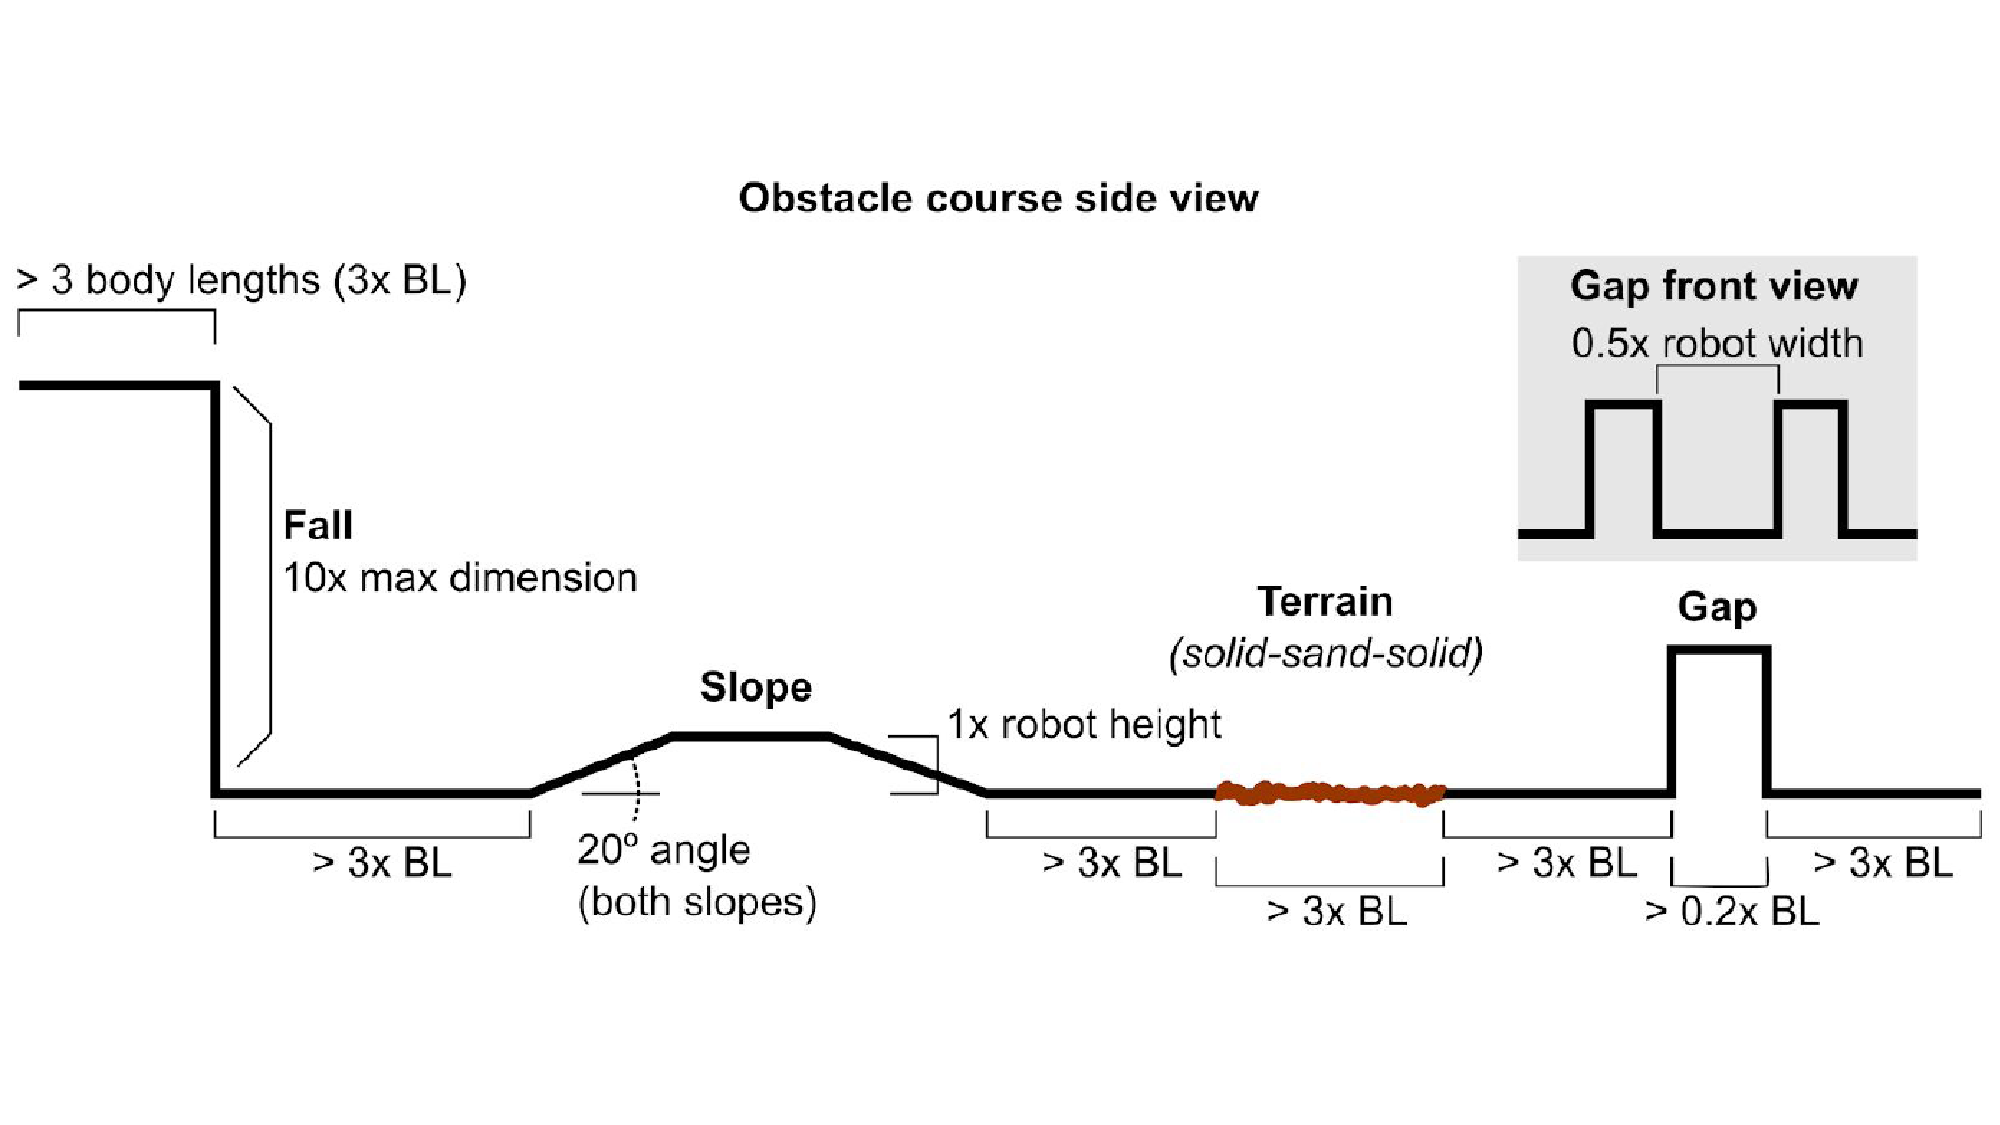
\includegraphics[width=0.7\textwidth]{sorocomp.pdf}
    \caption[]{}
    \label{fig:sorocomp}
\end{figure}